\section{Linux History}

\begin{frame}
   {Linux History}
   \begin{multicols}{2}
      \begin{figure}[H]
         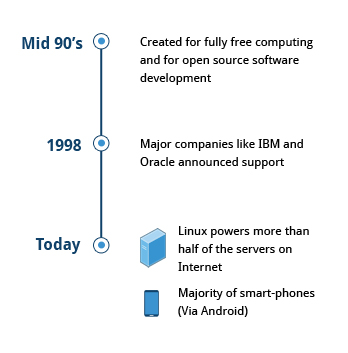
\includegraphics[width=2.2in]{IMAGES/linuxhistory}
         \caption{Linux Adoption History}
      \end{figure}
      \begin{itemize}
         \item Created 1991, by Linus Torvalds
         \item Vendors provided support starting in mid-90's
         \item Major companies announced support (1998)
         \begin{itemize}
            \item \textbf{IBM}, \textbf{Compaq}, \textbf{Oracle}
         \end{itemize}

         \item Present: widespread adoption
         \begin{itemize}
            \item \textbf{Linux} kernel used everywhere
            \item Endless variety of \textbf{Linux} distributions
         \end{itemize}
         \item
         \textbf{Linux} handles:
         \begin{itemize}
            \item Dozens of architectures, both 32-bit and 64-bit
            \item From small embedded systems to vast majority of
            the world's supercomputers
         \end{itemize}
      \end{itemize}
   \end{multicols}


\end{frame}

\cprotect\note{

   \textbf{Linux} was first announced to the world on
   August 25, 1991, by Linus Torvalds, then a 21 year old
   student at The University of Helsinki, in a posting to a
   \textbf{Usenet} newsgroup, saying in part:

   \begin{quote}
      Hello everybody out there using minix -

      I'm doing a (free) operating system (just a hobby,
      won't be big and professional like gnu) for 386(486)
      AT clones. .....
   \end{quote}

   Linus' original motivation was to write a terminal
   emulator for the purpose of accessing the University's
   \textbf{UNIX} servers. He began using the \textbf{MINIX}
   operating system, but became frustrated by its licensing
   constraints, which limited it to educational use, and by
   the procedures for having changes made.


   The original release 0.01 was released under its own
   license, which had restrictions on commercial activity.
   In December 1992 version 0.99 was released under the
   \textbf{GNU GPL} under which it has remained ever since.

   The first really usable \textbf{Linux Distributions},
   \textbf{Slackware}, \textbf{Debian}, and the predecessor
   of \textbf{SuSe} were released in 1992; with \textbf{Red
   Hat} following in 1994. In the meantime the number of
   contributors to \textbf{Linux} development grew from a
   handful to hundreds and then to thousands.

   Corporate involvement in \textbf{Linux} has steadily
   grown, and was accelerated by a one billion dollar
   investment by \textbf{IBM} in 2000. Today while there
   are many independent developers contributing to
   \textbf{Linux}, a large share comes from both major
   \textbf{Linux} distributors, and major hardware and
   software industry players.

}

